\documentclass[tikz]{standalone}
\usetikzlibrary{arrows.meta, positioning, fit, shapes.misc}

\begin{document}
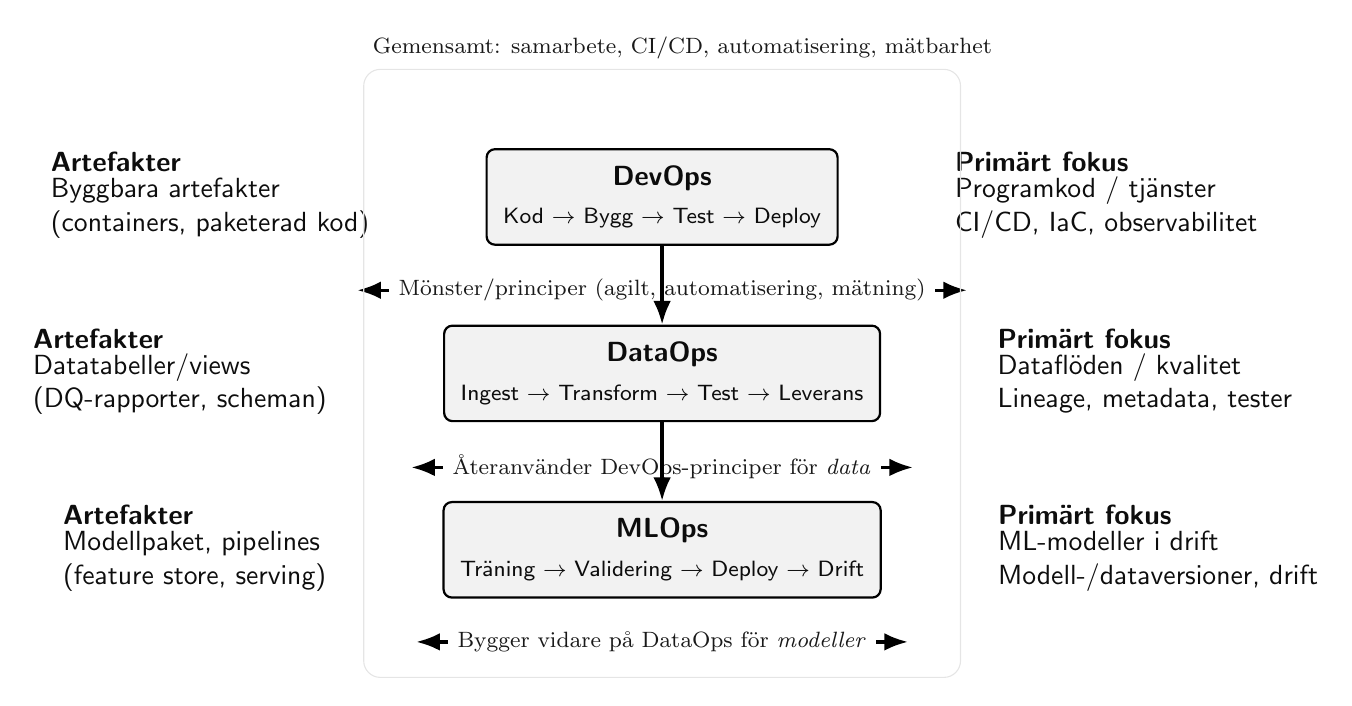
\begin{tikzpicture}[
  font=\sffamily,
  box/.style={rounded corners=3pt, draw, thick, inner sep=6pt, minimum width=36mm, align=center},
  arrow/.style={-{Latex[length=3mm]}, very thick},
  note/.style={align=left, inner sep=2pt},
  lbl/.style={font=\footnotesize, text opacity=0.9},
  every node/.style={text opacity=0.95}
]

% Main boxes (top->down)
\node[box, fill=gray!10] (devops) { \textbf{DevOps}\\[2pt]\footnotesize Kod $\rightarrow$ Bygg $\rightarrow$ Test $\rightarrow$ Deploy };
\node[box, fill=gray!10, below=10mm of devops] (dataops) { \textbf{DataOps}\\[2pt]\footnotesize Ingest $\rightarrow$ Transform $\rightarrow$ Test $\rightarrow$ Leverans };
\node[box, fill=gray!10, below=10mm of dataops] (mlops) { \textbf{MLOps}\\[2pt]\footnotesize Träning $\rightarrow$ Validering $\rightarrow$ Deploy $\rightarrow$ Drift };

% Flow arrows
\draw[arrow] (devops) -- (dataops);
\draw[arrow] (dataops) -- (mlops);

% Side notes (differences / focus)
\node[note, right=14mm of devops] (d1) {
  \textbf{Primärt fokus}\\
  \begin{tabular}{@{}l@{}}
  Programkod / tjänster\\
  CI/CD, IaC, observabilitet
  \end{tabular}
};
\node[note, right=14mm of dataops] (d2) {
  \textbf{Primärt fokus}\\
  \begin{tabular}{@{}l@{}}
  Dataflöden / kvalitet\\
  Lineage, metadata, tester
  \end{tabular}
};
\node[note, right=14mm of mlops] (d3) {
  \textbf{Primärt fokus}\\
  \begin{tabular}{@{}l@{}}
  ML-modeller i drift\\
  Modell-/data\-versioner, drift
  \end{tabular}
};

% Left side: typical artifacts/outputs
\node[note, left=14mm of devops] (a1) {
  \textbf{Artefakter}\\
  \begin{tabular}{@{}l@{}}
  Byggbara artefakter\\
  (containers, paketerad kod)
  \end{tabular}
};
\node[note, left=14mm of dataops] (a2) {
  \textbf{Artefakter}\\
  \begin{tabular}{@{}l@{}}
  Datatabeller/views\\
  (DQ-rapporter, scheman)
  \end{tabular}
};
\node[note, left=14mm of mlops] (a3) {
  \textbf{Artefakter}\\
  \begin{tabular}{@{}l@{}}
  Modellpaket, pipelines\\
  (feature store, serving)
  \end{tabular}
};

% Brackets that show “builds on”
\node[below=3mm of devops, lbl] (l1) {Mönster/principer (agilt, automatisering, mätning)};
\draw[arrow, shorten >=2mm] (l1.west) -- ++(-6mm,0);
\draw[arrow, shorten >=2mm] (l1.east) -- ++(6mm,0);

\node[below=3mm of dataops, lbl] (l2) {Återanvänder DevOps-principer för \textit{data}};
\draw[arrow, shorten >=2mm] (l2.west) -- ++(-6mm,0);
\draw[arrow, shorten >=2mm] (l2.east) -- ++(6mm,0);

\node[below=3mm of mlops, lbl] (l3) {Bygger vidare på DataOps för \textit{modeller}};
\draw[arrow, shorten >=2mm] (l3.west) -- ++(-6mm,0);
\draw[arrow, shorten >=2mm] (l3.east) -- ++(6mm,0);

% Optional faint group boxes to imply nesting
\node[draw, rounded corners=6pt, fit=(devops) (dataops) (mlops), inner sep=10mm, draw=black!10] (frame) {};
\node[above right=0mm and 0mm of frame.north west, anchor=south west, lbl] {\footnotesize Gemensamt: samarbete, CI/CD, automatisering, mätbarhet};

\end{tikzpicture}
\end{document}
